\chapter{Comunicazione con sincronizzazione estesa}

\section{Semantica}

La comunicazione con sincronizzazione estesa è un modello di \textbf{comunicazione}/\textbf{estesa} in cui:
\begin{itemize}
    \item il processo mittente richiede l'esecuzione di un \textbf{servizio} al processo destinatario
    \item il processo mittente rimane \textbf{sospeso} fino al competamente del servizio richiesto
\end{itemize}

I processi rimangono \textit{sincronizzati} durante l'esecuzione del servizio da parte del ricevente fino alla \textit{ricezione dei risultati} da parte del mittente.

Il meccanismo è noto anche con il nome di \textbf{chiamata di operazione remota}.

Esiste una forte analogia con una classica chiamata a funzione, dove il chiamante attende il completamento dell'operazione prima di proseguire.

La differenza sostanziale è che l'operazione viene eseguita \textbf{remotamente} da un processo diverso dal chiamante.


\section{Implementazione}

Esistono due modalità diverse di implementazione lato server:
\begin{itemize}
    \item chiamata di procedura remota \textbf{RPC}
    \item \textbf{rendez-vous esteso}
\end{itemize}

\subsection{Chiamata di procedura remota}

Per ogni operazione che un processo client può ricevere viene dichiarata, lato server, una \textbf{procedura}.

Per ogni richiesta di operazione al server, viene creato un \textbf{nuovo processo} (thread) che ha il compito di eseguire la procedura corrispondente.

\begin{figure}[H]
    \centering
    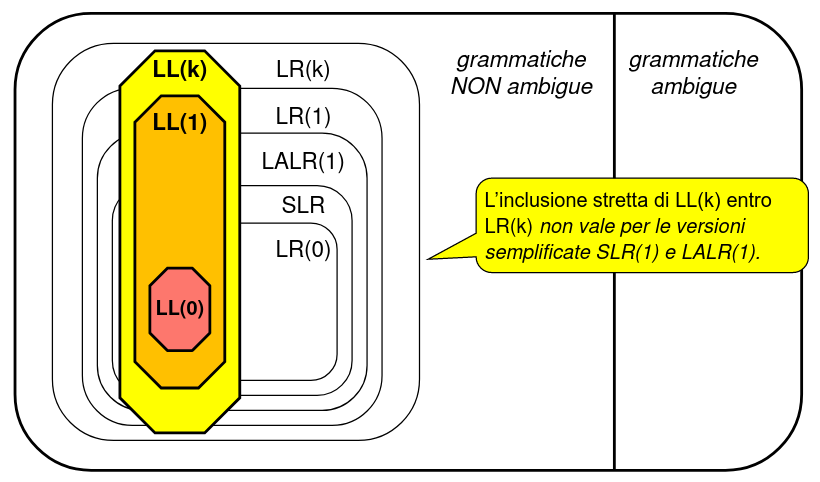
\includegraphics[width=0.6\textwidth]{/home/riccardoob/appunti/sistemi_operativi/images/47.png}
\end{figure}

\subsection{Rendez vous}

L'operazione richiesta viene specificata come un \textbf{insieme di istruzioni} che può comparire in un punto qualunque del processo servitore (linguaggio ADA).

Il processo servitore utilizza un'istruzione di input (\texttt{accept}) che lo sospende in attesa di una richiesta dell'operazione.

All'arrivo della richiesta il servitore esegue il corretto insieme di istruzioni e invia i risultati al chiamante.

\begin{figure}[H]
    \centering
    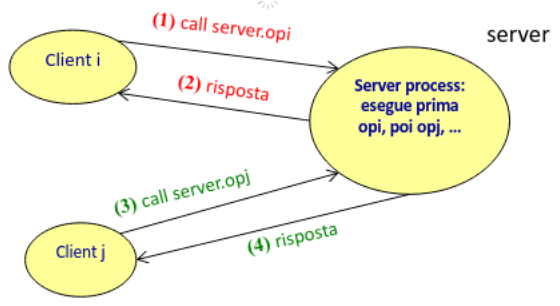
\includegraphics[width=0.6\textwidth]{/home/riccardoob/appunti/sistemi_operativi/images/48.png}
\end{figure}

\subsection{RPC vs rendez-vous}

\subsubsection{RPC}
Rappresenta solo un \textit{meccanismo di \textbf{comunicazione} tra processi}: la possibilità che più operazioni siano eseguite concorrentemente implica la necessità di sincronizzazione tra i vari processi servitori (a carico del programmatore).

\subsubsection{Rendez-vous esteso}
Combina \textbf{combinazione} con \textbf{sincronizzazione}, esiste un solo processo servitore al cui interno sono definite le istruzioni che consentono di realizzare il servizio richiesto. Il processo servitore si sincronizza con il processo cliente quando esegue l'operazione di \texttt{accept}.

\subsection{Chiamata di procedura remota}

L'insieme delle procedure remote è definito all'interno di un componente software, \textbf{modulo}, che contiene anche le variabili locali al server ed eventuali procedure e processi locali.

\begin{minted}[bgcolor=lightgray,framesep=2mm,baselinestretch=1.2,fontsize=\footnotesize,escapeinside=||,mathescape=true]{c}
//server
module nome_del_modulo {
    <dichiarazione delle variabili locali>;
    <inizializzazione delle variabili locali>;
    public void op1 (<parametri formali>){
    <corpo della procedura op1>;}
    ...
    public void opn (<parametri formali>){
    <corpo della procedura opn >;}
    <dichiarazione di procedure locali>;
    <dichiarazione di processi locali>;
}
\end{minted}

I singoli moduli operano su \textit{spazi di indirizzamento diversi} e possono quindi essere \textit{allocati su nodi distinti della rete}.

La chiamata di una procedura remota verrà specificata dal client con uno statement del tipo:

\begin{minted}[bgcolor=lightgray,framesep=2mm,baselinestretch=1.2,fontsize=\footnotesize,escapeinside=||,mathescape=true]{c}
module client {
    //...
    call nome_del_modulo.op_i (<parametri attuali>);
    //...
\end{minted}

A ogni istante è possibile che più \textit{thread concorrenti} all'interno del modulo server accedano a variabili interne, è quindi necessaria \textbf{sincronizzazione} (monitor, semafori...).

\subsubsection{Esempio - servizio di sveglia}
Server
\begin{minted}[bgcolor=lightgray,framesep=2mm,baselinestretch=1.2,fontsize=\footnotesize,escapeinside=||,mathescape=true]{c}
module allarme {
    int time;
    semaphore mutex = 1;
    semaphore priv[N] = 0; //sem privati sospensione processi
    coda_richieste coda; //struttura richieste di sveglia
    
    public void richiesta_sveglia(int timeout, int id) {
        int sveglia = time + timeout;
        P(mutex);
        <inserimento sveglia e id nella coda di risveglio
        matenendo ordinata con id non decrescenti>
        V(mutex);
        P(priv[id]); //attesa sveglia
    }
    
    process clock { //demone
        int tempo_di_sveglia;
        <avvia il clock>;
        while (true) {
            <attende interruzione, quindi riavvia il clock>;
            time++;
            P(mutex);
            tempo_di_sveglia = <min valore di sveglia in coda>;
            while (time >= tempo_di_sveglia) {
                <rimozione di tempo_di_sveglia e id da coda>;
                V(priv[id]);
            }
            V(mutex);
        }
    }
}
\end{minted}
Client
\begin{minted}[bgcolor=lightgray,framesep=2mm,baselinestretch=1.2,fontsize=\footnotesize,escapeinside=||,mathescape=true]{c}
call allarme.richiesta_sveglia(60); //crea thread dedicato nel server
\end{minted}

\begin{figure}[H]
    \centering
    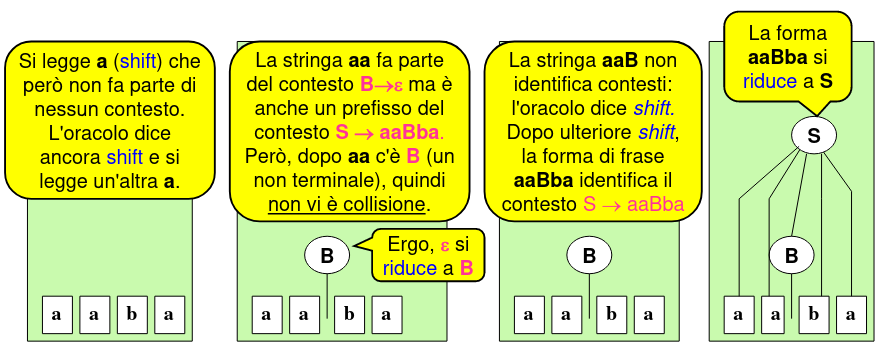
\includegraphics[width=0.5\textwidth]{/home/riccardoob/appunti/sistemi_operativi/images/49.png}
\end{figure}

\subsection{Rendez vous esteso}
Il servizio richiesto viene specificato dal server come un insieme di istruzioni che può comparire in un qualsiasi punto del processo del server tremite una \texttt{accept}.

\begin{minted}[bgcolor=lightgray,framesep=2mm,baselinestretch=1.2,fontsize=\footnotesize,escapeinside=||,mathescape=true]{ada}
accept <servizio>(in <par-ingresso>, out <par-uscita>) -> {S1, ..., S_n}
\end{minted}

Il client richiede il servizio con l'istruzione
\begin{minted}[bgcolor=lightgray,framesep=2mm,baselinestretch=1.2,fontsize=\footnotesize,escapeinside=||,mathescape=true]{ada}
call <server>.<servizio>(<parametri attuali>);
\end{minted}

\subsubsection{Accept}
Semantica dell'operazione accept:
\begin{itemize}
    \item se non sono presenti richieste del servizio S è sospensiva
    \item se S viene richiesto da più processi, vengono evasi in politica FIFO
    \item a uno stesso servizio possono essere associate più accept nel codice eseguito dal server: a un richiesta possono corrispondere azioni diverse
    \item lo schema di comunicazione è di tipo \textbf{asimmetrico molti a uno}
\end{itemize}

Possibili sequenze di comunicazione
\begin{multicols}{2}
\begin{multicolfigure}
    \centering
    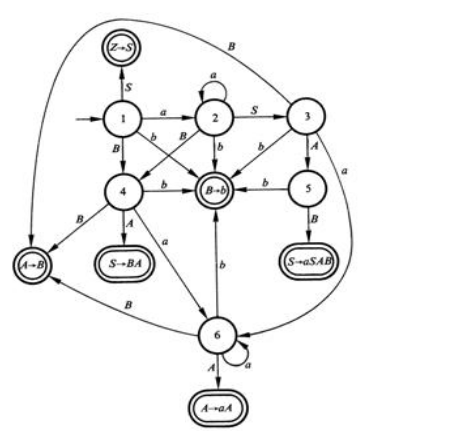
\includegraphics[width=\textwidth]{/home/riccardoob/appunti/sistemi_operativi/images/50.png}
\end{multicolfigure}
\columnbreak
\begin{multicolfigure}
    \centering
    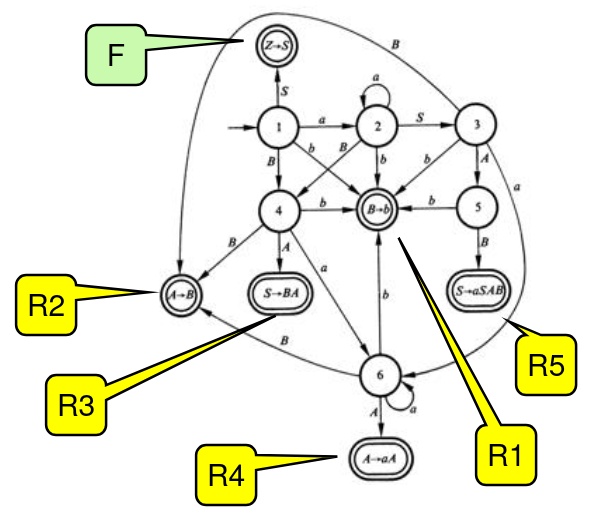
\includegraphics[width=\textwidth]{/home/riccardoob/appunti/sistemi_operativi/images/51.png}
\end{multicolfigure}
    
\end{multicols}

\noindent
Selezione delle richieste:

Nel modello rendez-vous le richieste vengono scelte a seconda del suo stato interno, utilizzando comandi con guardia:
\begin{minted}[bgcolor=lightgray,framesep=2mm,baselinestretch=1.2,fontsize=\footnotesize,escapeinside=||,mathescape=true]{go}
select
    [] <stato1>; accept <servizio1>(in <par-ingresso>, out<par-uscita>)
        -> {S11, ..., S1n}; ...
    [] <stato2>; accept <servizio2>(in <par-ingresso>, out<par-uscita>)
        -> {S21, ..., S2n}; ...
    ...
end;
\end{minted}

\subsubsection{Esempio - produttore e consumatore, buffer capacità N}
\begin{minted}[bgcolor=lightgray,framesep=2mm,baselinestretch=1.2,fontsize=\footnotesize,escapeinside=||,mathescape=true]{go}
process buffer { //server
    messaggio buff[N];
    int testa = 0, coda = 0;
    int cont = 0;
    do {
        [] (cont < N); accept inserisci(in dato:messaggio) ->
            { buff[coda] = dato; } //fine rendez-vous
            cont++;
            coda = (coda + 1) % N;
        [] (cont > 0); accept preleva(out dato:messaggio) ->
            { dato = buff[testa]; } //fine rendez-vous
            cont--;
            testa = (testa + 1) % N;
    }
}
\end{minted}
La sincronizzazione tra client e server è limitata alle sole \textit{istruzioni comprese nel blocco di accept} (dentro \{...\}).

\begin{minted}[bgcolor=lightgray,framesep=2mm,baselinestretch=1.2,fontsize=\footnotesize,escapeinside=||,mathescape=true]{go}
process produttore_i {
    messaggio dati;
    for (;;) {
        <produci dati>;
        call buffer.inserisci(dati);
    }
}

process consumatore_j {
    messaggio dati;
    for (;;) {
        call buffer.preleva(dati);
        <consuma dati>;
    }
}
\end{minted}

\subsubsection{Selezione delle richieste in base ai parametri di ingresso}
La decisione di servizio può dipendere anche da \textbf{parametri} della richiesta stessa, oltre che allo stato della risorsa. 

Ciò non è possibile tramite la guardia di ingresso: è necessaria una \textbf{doppia interazione} tra client e server, prima per i parametri e poi per il servizio.

Nell'ipotesi di un \textit{numero limitato di differenti richieste} si può ottenere una semplice soluzione al problema associando ad ogni possibile richiesta una differente operazione.

In alcuni linguaggi è possibile aggregare richieste possibili in strutture di tipo vettore: \textbf{vettore delle operazioni di servizio}.

\subsubsection{Esempio - sveglia}
Si consideri il caso del server allarme con il compito di inviare una segnalazione di sveglia ad un insieme di processi che richiedono il servizio con un tempo da essi stabilito.

Server, tre tipi di richiesta:
\begin{itemize}
    \item \textbf{tick}: aggiornamento del tempo
    \item \textbf{richiesta\_di\_sveglia(T)}: impostazione sveglia per il mittente
    \item \textbf{svegliami[T]}: attesa del segnale di allarma al tempo specificato
\end{itemize}

L'ordine con cui il processo allarme risponde alle richieste del tipo \texttt{svegliami} dipende solo dal parametro T comunicato con la richiesta.

Struttura generica cliente:
\begin{minted}[bgcolor=lightgray,framesep=2mm,baselinestretch=1.2,fontsize=\footnotesize,escapeinside=||,mathescape=true]{go}
process client_i {
    //...
    allarme.richiesta_di_sveglia(T);
    //...
    allarme.svegliami[T];
    //...
}
\end{minted}

Vettore di operazioni di servizio:
\begin{minted}[bgcolor=lightgray,framesep=2mm,baselinestretch=1.2,fontsize=\footnotesize,escapeinside=||,mathescape=true]{go}
typedef struct {
    int risveglio;
    int intervallo;
} dati_di_risveglio;

dati_di_risveglio tempo_di_sveglia[N];
\end{minted}

Server:
\begin{minted}[bgcolor=lightgray,framesep=2mm,baselinestretch=1.2,fontsize=\footnotesize,escapeinside=||,mathescape=true]{go}
process allarme {
    entry tick;
    entry richiesta_di_sveglia(in int intervallo);
    entry svegliami[first..last]; //vettore operazioni

    int tempo;
    typedef struct {
        int risveglio;
        int intervallo;
    } dati_di_risveglio;
    dati_di_risveglio tempo_di_sveglia[N];

    do {
        [] accept tick; -> {tempo++;}
        [] accept richiesta_di_sveglia(in int intervallo)
            ->
\end{minted}

